\chapter{Improvements}
\label{chapter:improvements}

\section{Automation}

Using the study plug-in a mixing engineer will not have to draw gain automations manually. Nevertheless it can be useful to have an automation drawn by the plug-in. On one hand side it visualises the adapted gain curve better than the gain slider contained in the UI alone. On the other hand, it can save up calculation resources when the plug-in reads its own automation instead of processing the same vocal track in a repeated way. This is not necessary in simple mixing sessions but comes in handy when the mixed musical piece contains a great number of tracks with even more digital effects on each channel. Every digital effect increases CPU power needs. Often single tracks are bounced in place\footnote{all effects are rendered and combined with the actual signal to a new audio file} to avoid problems in performance. When the plug-in just reads an automation it is no considerable part of this problem even if there are multiple vocal tracks using this effect.\\
For those reasons the study plug-in was extended with this feature supported by the JUCE framework (see chapter \ref{chapter:realization}.3).
The final solution sets a automation point every 80ms as long the gain changed about at least 0.1dB. Therefore the gain adaption is constantly drawn in the automation curve but 12,5 instead of 41000 times a second or more. It does not set a new point when the gain is not adapting as this would be redundant.\\

\section{Adapting Loudness Goal}

The $L_{goal}$ parameter is not regarded as a gain controller. It is not designed to amplify the signal to a desired level. Instead, it should be adjusted to the actual loudness of the signal. In this way the plug-in can use its full range for changes on dynamics. For example when $L_{goal}$ is set far below the signal level, the plug-in will stay at its minimal allowed gain value (initalized with -6dB) as long as it gets the high-level input. Even if it is at one end of the user defined dynamic range it will still operate in half (only negative/positive gain adaption) for most of the time. Therefore it is important to set $L_{goal}$ correctly. In best practice the plug-in will compress the incoming signal as much as amplifying it.\\
A user is able to set $L_{goal}$ according to the vocal level. However, it still remains a problem as the perfect loudness goal possibly alters through a song. As a consequence it is difficult for a human to guess the average setting for the entire musical piece. Therefore some calculation-based solutions were tested.\\
The first approach was determining a new $L_{goal}$ for every second. To achieve this the plug-in summed up all resulting gain values for each sample in this time period. Afterwards it calculated the average tendency (more positive or more negative gain values). The offset was finally subtracted from the current $L_{goal}$ and the sum of the gain values got reset.\\
Problematic with this approach was that the $L_{goal}$ adaption was one second too late if the signal level changed. In addition it diminished some advantages of the plug-in as it treated different parts of the vocals with different settings which results in some local benefits but leads to varying level through the whole track.\\
As a consequence analysing only parts of the vocal track would not lead to a profitable result. Furthermore, the plug-in should go through all critical parts of its input and therefore decide for the best suiting $L_{goal}$. In conclusion $L_{goal}$-detection was implemented. During the time this detection algorithm is active, the plug-in will not multiply the calculated gain with the signal but is still determining it, dissimilar to a regular bypass. In addition the plug-in re-adjusts its allowed gain range for this period of time to the maximum (+/- 10dB). This is performed to find the most accurate average loudness rate and it has no negative consequences as it endures as long as the detection is processing. If the plug-in runs the detection through the full vocal track it calculates a decent $L_{goal}$. To avoid the result being falsified by sections without vocal signal, it only adapts on input with actual signal.\\
This is a task predestined to be performed offline, but due to the complexity of offline calculations in a plug-in operating in different DAWs the resources to realise it were not available in this study. For future work it would be possible to make use of the full ITU-R BS.1770-4\cite{ITUalgo} algorithm for this task.\\
Although the $L_{goal}$-detection algorithm is probably the best current way to set the parameter, it is still allowed for a user to choose it manually for own creative reasons.\\
When $L_{goal}$ algorithmically adapts or is set to a new value chosen by the user the threshold of the plug-ins gate will change as well. Regardless of whether the average input is of low or high level the plug-in is thus able to handle it with reasonable settings.\\

\section{Side Chain}

So far the plug-in works well on single audio tracks and reduces long term dynamics. This substantially lessens the work for a mixing engineer but a average vocal level staying constant during a whole musical piece is not necessarily the wanted result. If the instrumental backtracks varies in loudness it is desirable for the plug-in to vary its output gain accordingly. To realise this variation the plug-in requires additional information. Therefore a side chain input was added to the plug-in's interface.\\
After implementing the new input this information had to be processed. This information about the loudness of the backtrack (to be fed into the side chain) is needed to enable determination of a useful additional output gain. In process of detecting the loudness of the side chain input the additional signal is passing through the filter, through RMS and gain calculations as the regular input signal (see Fig. \ref{Chain2}). Passing includes transformation into logarithmic number space. Afterwards the signal is compared to the current $L_{goal}$ and the calculated difference is smoothed. Now the smoothed gain is transferred back to linear number space and it is multiplied with the gain of the parallel determination from the main input.\\
It is important for the side chain processing not to interfere with the main input gain calculations of the plug-in. Especially $L_{goal}$ must not be changed through this process. Otherwise it would corrupt its results in terms of dynamic range and make the $L_{goal}$ detection useless.\\
While testing in real use cases it was found beneficial to add an additional output gain for the finally returned signal. This reduced the effort of matching vocal output level with the backtrack. It would be an advantage if the plug-in could set the output gain itself depending on the side chain input, but as for different music styles and creative decisions there is not one correct version of vocal-to-backtrack relation but a great number of reasonable options could be appropriate. Nevertheless during future improvements of the plug-in this part could be simplified in its user interaction.\\
A remaining question for the side chain implementation related to setting of the average time coefficients for RMS calculations and gain adaption (see chapter \ref{chapter:realization}.1). On one hand side it should not react on small changes (for example when a musician is just accentuating certain beats in the backtrack), on the other hand side it needs to react fast enough to calculate an appropriate gain for the first words of a new song part with a different loudness level. It is not negligible that it operates with the lookahead already realised for the plug-ins main use.\\
Additionally, in the first approach it turned out to be a difficult problem for the side chain gain adaption to deal with instrumental breaks of longer duration (up to a full bar). While most of the instruments are pausing during those breaks the vocals should stay at the same level as it is often used to emphasize the remaining musicians. With the current implementation of side chain adaption instrumental breaks were causing a parallel slowly falling vocal level. After the implementation of the idle time (see below) at gain adaption this behaviour could be avoided for the most part.\\

\begin{figure}
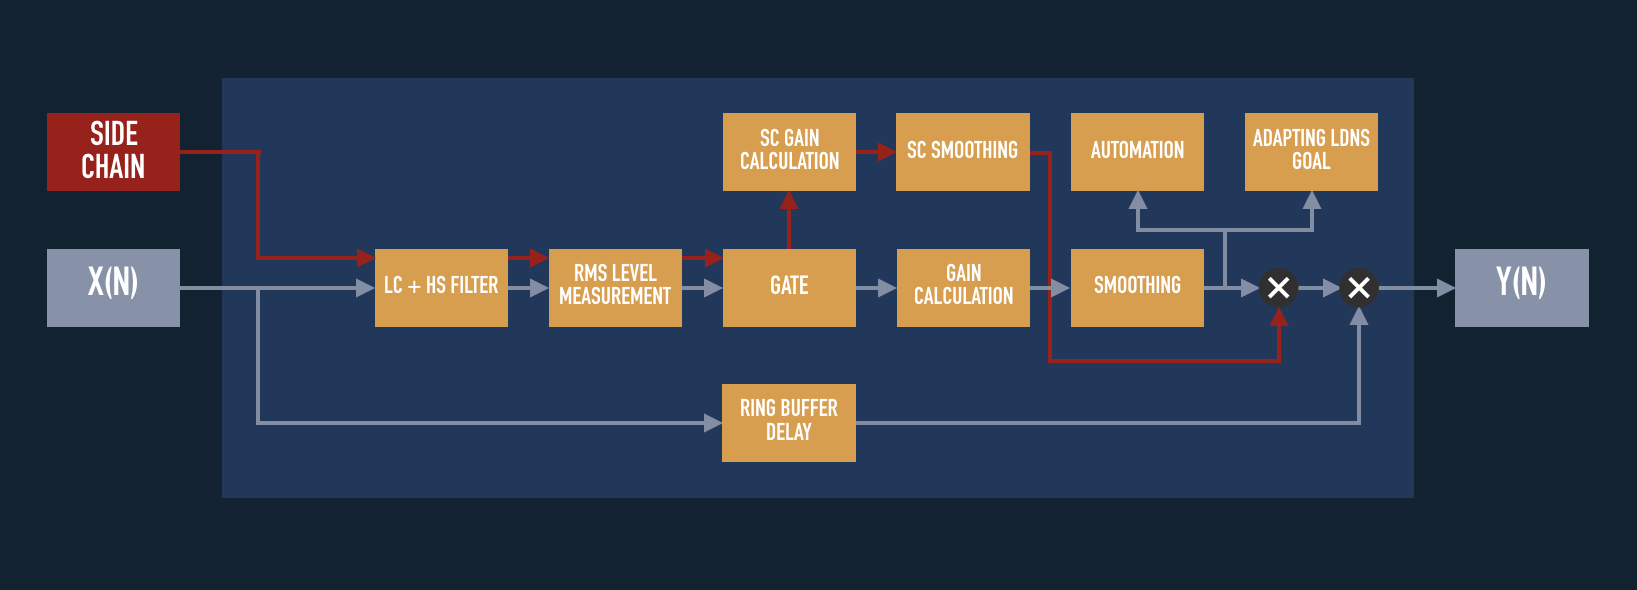
\includegraphics[width=\textwidth]{images/chain02}
\caption{Improved processing chain}
\label{Chain2}
\end{figure}

\section{Idle Time}

'Idle time' describes the time the plug-in will wait with further gain adaption when the input level falls below a certain threshold. The effect of an idle time is that the plug-in will ignore short gaps between vocal signals. Therefore the plug-in does not change the adapted gain for example when a singer does a short rhythmic break in his/her vocals. So it will just use the actual vocals in the input for gain adaption similar to how a mixing engineer would do it. Due to a reasonable short duration of the idle time it is still able to adapt to 0dB gain for parts without singing. Subsequently there will be no risk of amplifying unwanted noise. The short period after a vocal signal and before a part of silence were the plug-in is still idle will not remain much longer than the vocal decay and is even shortened by the amount of lookahead delay.\\
At the first approach in implementing this feature the function of the gate was expanded. Each time the input dropped below threshold, the current sample was replaced by the last one above threshold during the set amount of idle time. Due to the fact that the last sample above threshold is still being at comparably low level it did not work as expected. The subsequent gain adapting was consequently falling to even lower results than without the change at the gate because at idle time it got values near the lowest possible one which was just not set to $L_{goal}$ by the gate. It is assumed that the error could be fixed by replacing the samples at idle time with a RMS value from a sample further ahead, but this would require a additional memory space for past samples and it seemed to be too complex for this study.\\
Therefore, the current implementation is based on the plan that the plug-in should detect previously to the gain adaption whether there is no vocal signal and then freeze the current gain. As the gain adaption is much slower due to compress/amplification time smoothing than the RMS averaging before the gate, it therefore freezes the gain value before it is able to adapt to the level change.\\
The algorithm detects whether the current level is below gate threshold by comparing the sample with $L_{goal}$. If the transferred RMS averaged sample is at the exact value of $L_{goal}$ it can be assumed that the gate replaced its actual value. The rare case of a sample being randomly at exact the level of $L_{goal}$ and therefore stop the gain adaption cannot be eliminated in this implementation. Nevertheless, this makes no noticeable difference as it just stops the slow gain adaption for one single sample (max 1/44100 sec in expected use case). At the first sample differing from $L_{goal}$ the idle timer is reset and the gain adaption continuous. When the maximum idle time is reached it has the same effect apart from resetting the idle time counter.\\
With the idle time working well in the main processing chain of the plug-in, its advantages in terms of side chain integration were evaluated. With the plug-in version developed so far there was still a problem related to instrumental breaks and their unwanted impact on the calculated gain correction. Therefore a implementation of idle time similar to the already existing one for the main input was used. At the final side chain calculations it was implemented and adjusted the length of the maximum idle time with tests in a real mixing environment. The result with a reasonable set maximum was quite acceptable as it substantially reduced the gain drop during instrumental breaks as long as the side chain input level was adapted to $L_{goal}$. For better adjustment of side chain-to-$L_{goal}$ relation, an additional input gain for the side chain was implemented. As it remains difficult to adjust it correctly for a whole song a self setting algorithm for the input gain was added similar to the already existing $L_{goal}$ detection. As mentioned earlier this would be significantly better realised in an offline thread but also works in real time for now.\\

\begin{figure}
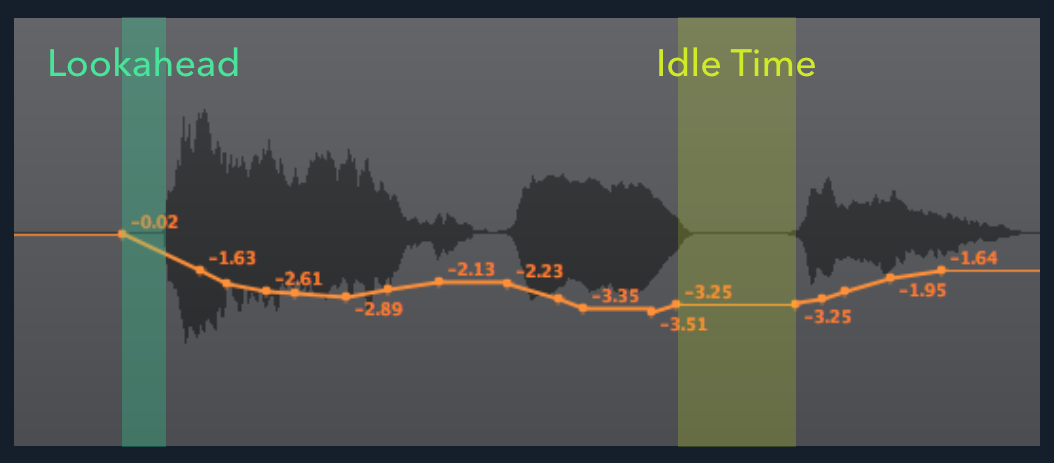
\includegraphics[width=0.8\textwidth]{images/automation2LookIdle}
	\centering
	\caption{Idle time and lookahead marked at automation written by the study plug-in}
	\label{auto2look}
\end{figure}

\section{Wet/Dry}

Many plug-in effects for DAWs have an additional slider to adjust the wet/dry ratio of their outcome. In these terms 100\% “dry” is similar to the signal without the effect and 100\% “wet” is a fully processed effect on the signal. This reduces the effort which would be necessary for sending the signal on a second track with the effect inserted to mix both tracks together in wanted proportions.\\
In consideration of the use of such a slider in the plug-in of this study, it seemed useful at first as it enables a user to set the intensity of dynamic compression. On the other hand this is already possible in a slightly different way with better outcome, by changing the current gain range. In addition that this feature has its main use in creative work, which is not the main objective of this plug-in, the final plug-in will not include a wet/dry slider for now. This decision was made with the intention to simplify the final UI to its foundation followed by the reduction of the settable parameters (see chapter \ref{chapter:realization}.1).\\

\section{Final Gain Clipping}

Due to the problems of a possible disproportional gain (see chapter \ref{chapter:prototype}.6) caused by an unexpected error, it needs to be checked before it is finally multiplied with the plug-in’s input signal. This includes the gain of the plug-ins main functionality, the additional side chain gain and the user set output gain. It is not easy to set a good clip range\footnote{maximal and minimal determined gain value} as with 3 different gain values multiplied it can result in problematically high amplification which can be on purpose in some cases. In todays DAWs usually clipping at 1.0 in linear number space is only happening at the master fader. As consequence it is unproblematic to mix a single audio track above this threshold as long as the final mix will happen below. Therefore it is not reasonable to clip the gain*input product for +/- 1.0 sample values.\\
As consequence not the final outcome could be clipped but the final multiplied gain which includes all three gain variables. The clip was set to operate in the linear number space as last instance before the final multiplication. It clips the final gain for the range of 0.0 to 6.0. The clipping range starts at 0.0 because negative gain in the linear number space does not make sense in this context as it would only invert the phase of the input signal in addition to the compression or amplification. 6.0 is the clip in terms of amplification which is similar to a approximately 15dB gain boost. This is lower than the highest value that can be achieved with all gain sliders on maximum setting but this is not expected to happen in reasonable use. With a clip at 6.0 the input signal could be amplified by 600\%. If a signal needs stronger amplification in professional mixing it is presumable that the setting was done wrong or the recording is bad and should be replaced. If this could not be done or is not wanted it is necessary to edit the audio track before the start of the mixing session as the plug-in is not able to handle it alone. Since this case is still unlikely to occur in professional mixing the plug-in stays within the safety clipping range that will fit its intended use cases.\\